%!TEX program = xelatex
%% bare_jrnl_transmag.tex
%% V1.4
%% 2012/12/27
%% by Michael Shell
%% see http://www.michaelshell.org/
%% for current contact information.
%%
%% This is a skeleton file demonstrating the use of IEEEtran.cls
%% (requires IEEEtran.cls version 1.8 or later) with an IEEE 
%% Transactions on Magnetics journal paper.
%%
%% Support sites:
%% http://www.michaelshell.org/tex/ieeetran/
%% http://www.ctan.org/tex-archive/macros/latex/contrib/IEEEtran/
%% and
%% http://www.ieee.org/



% *** Authors should verify (and, if needed, correct) their LaTeX system  ***
% *** with the testflow diagnostic prior to trusting their LaTeX platform ***
% *** with production work. IEEE's font choices can trigger bugs that do  ***
% *** not appear when using other class files.                            ***
% The testflow support page is at:
% http://www.michaelshell.org/tex/testflow/


%%*************************************************************************
%% Legal Notice:
%% This code is offered as-is without any warranty either expressed or
%% implied; without even the implied warranty of MERCHANTABILITY or
%% FITNESS FOR A PARTICULAR PURPOSE! 
%% User assumes all risk.
%% In no event shall IEEE or any contributor to this code be liable for
%% any damages or losses, including, but not limited to, incidental,
%% consequential, or any other damages, resulting from the use or misuse
%% of any information contained here.
%%
%% All comments are the opinions of their respective authors and are not
%% necessarily endorsed by the IEEE.
%%
%% This work is distributed under the LaTeX Project Public License (LPPL)
%% ( http://www.latex-project.org/ ) version 1.3, and may be freely used,
%% distributed and modified. A copy of the LPPL, version 1.3, is included
%% in the base LaTeX documentation of all distributions of LaTeX released
%% 2003/12/01 or later.
%% Retain all contribution notices and credits.
%% ** Modified files should be clearly indicated as such, including  **
%% ** renaming them and changing author support contact information. **
%%
%% File list of work: IEEEtran.cls, IEEEtran_HOWTO.pdf, bare_adv.tex,
%%                    bare_conf.tex, bare_jrnl.tex, bare_jrnl_compsoc.tex,
%%                    bare_jrnl_transmag.tex
%%*************************************************************************

% Note that the a4paper option is mainly intended so that authors in
% countries using A4 can easily print to A4 and see how their papers will
% look in print - the typesetting of the document will not typically be
% affected with changes in paper size (but the bottom and side margins will).
% Use the testflow package mentioned above to verify correct handling of
% both paper sizes by the user's LaTeX system.
%
% Also note that the "draftcls" or "draftclsnofoot", not "draft", option
% should be used if it is desired that the figures are to be displayed in
% draft mode.
%
\documentclass[journal,transmag]{IEEEtran}
\usepackage[utf8]{inputenc} % Required for inputting international characters
\usepackage[T1]{fontenc} % Output font encoding for international characters
\usepackage{mathpazo} % Use the Palatino font
\usepackage{graphicx} % Required for including images
\usepackage{booktabs} % Required for better horizontal rules in tables
\usepackage{listings} % Required for insertion of code
\usepackage{enumerate} % To modify the enumerate environment
\usepackage{ctex} % Chinese
\usepackage{setspace} % 行间距
\usepackage{indentfirst} % 首行缩进
\usepackage{ragged2e} % 两端对齐
\usepackage{color} % 颜色
\usepackage{hyperref} % 链接
\usepackage{listings}
\usepackage{multirow}
\usepackage{makecell}
%
% If IEEEtran.cls has not been installed into the LaTeX system files,
% manually specify the path to it like:
% \documentclass[journal]{../sty/IEEEtran}





% Some very useful LaTeX packages include:
% (uncomment the ones you want to load)


% *** MISC UTILITY PACKAGES ***
%
%\usepackage{ifpdf}
% Heiko Oberdiek's ifpdf.sty is very useful if you need conditional
% compilation based on whether the output is pdf or dvi.
% usage:
% \ifpdf
%   % pdf code
% \else
%   % dvi code
% \fi
% The latest version of ifpdf.sty can be obtained from:
% http://www.ctan.org/tex-archive/macros/latex/contrib/oberdiek/
% Also, note that IEEEtran.cls V1.7 and later provides a builtin
% \ifCLASSINFOpdf conditional that works the same way.
% When switching from latex to pdflatex and vice-versa, the compiler may
% have to be run twice to clear warning/error messages.






% *** CITATION PACKAGES ***
%
%\usepackage{cite}
% cite.sty was written by Donald Arseneau
% V1.6 and later of IEEEtran pre-defines the format of the cite.sty package
% \cite{} output to follow that of IEEE. Loading the cite package will
% result in citation numbers being automatically sorted and properly
% "compressed/ranged". e.g., [1], [9], [2], [7], [5], [6] without using
% cite.sty will become [1], [2], [5]--[7], [9] using cite.sty. cite.sty's
% \cite will automatically add leading space, if needed. Use cite.sty's
% noadjust option (cite.sty V3.8 and later) if you want to turn this off
% such as if a citation ever needs to be enclosed in parenthesis.
% cite.sty is already installed on most LaTeX systems. Be sure and use
% version 4.0 (2003-05-27) and later if using hyperref.sty. cite.sty does
% not currently provide for hyperlinked citations.
% The latest version can be obtained at:
% http://www.ctan.org/tex-archive/macros/latex/contrib/cite/
% The documentation is contained in the cite.sty file itself.






% *** GRAPHICS RELATED PACKAGES ***
%
\ifCLASSINFOpdf
  % \usepackage[pdftex]{graphicx}
  % declare the path(s) where your graphic files are
  % \graphicspath{{../pdf/}{../jpeg/}}
  % and their extensions so you won't have to specify these with
  % every instance of \includegraphics
  % \DeclareGraphicsExtensions{.pdf,.jpeg,.png}
\else
  % or other class option (dvipsone, dvipdf, if not using dvips). graphicx
  % will default to the driver specified in the system graphics.cfg if no
  % driver is specified.
  % \usepackage[dvips]{graphicx}
  % declare the path(s) where your graphic files are
  % \graphicspath{{../eps/}}
  % and their extensions so you won't have to specify these with
  % every instance of \includegraphics
  % \DeclareGraphicsExtensions{.eps}
\fi
% graphicx was written by David Carlisle and Sebastian Rahtz. It is
% required if you want graphics, photos, etc. graphicx.sty is already
% installed on most LaTeX systems. The latest version and documentation
% can be obtained at: 
% http://www.ctan.org/tex-archive/macros/latex/required/graphics/
% Another good source of documentation is "Using Imported Graphics in
% LaTeX2e" by Keith Reckdahl which can be found at:
% http://www.ctan.org/tex-archive/info/epslatex/
%
% latex, and pdflatex in dvi mode, support graphics in encapsulated
% postscript (.eps) format. pdflatex in pdf mode supports graphics
% in .pdf, .jpeg, .png and .mps (metapost) formats. Users should ensure
% that all non-photo figures use a vector format (.eps, .pdf, .mps) and
% not a bitmapped formats (.jpeg, .png). IEEE frowns on bitmapped formats
% which can result in "jaggedy"/blurry rendering of lines and letters as
% well as large increases in file sizes.
%
% You can find documentation about the pdfTeX application at:
% http://www.tug.org/applications/pdftex




% *** MATH PACKAGES ***
%
%\usepackage[cmex10]{amsmath}
% A popular package from the American Mathematical Society that provides
% many useful and powerful commands for dealing with mathematics. If using
% it, be sure to load this package with the cmex10 option to ensure that
% only type 1 fonts will utilized at all point sizes. Without this option,
% it is possible that some math symbols, particularly those within
% footnotes, will be rendered in bitmap form which will result in a
% document that can not be IEEE Xplore compliant!
%
% Also, note that the amsmath package sets \interdisplaylinepenalty to 10000
% thus preventing page breaks from occurring within multiline equations. Use:
%\interdisplaylinepenalty=2500
% after loading amsmath to restore such page breaks as IEEEtran.cls normally
% does. amsmath.sty is already installed on most LaTeX systems. The latest
% version and documentation can be obtained at:
% http://www.ctan.org/tex-archive/macros/latex/required/amslatex/math/





% *** SPECIALIZED LIST PACKAGES ***
%
%\usepackage{algorithmic}
% algorithmic.sty was written by Peter Williams and Rogerio Brito.
% This package provides an algorithmic environment fo describing algorithms.
% You can use the algorithmic environment in-text or within a figure
% environment to provide for a floating algorithm. Do NOT use the algorithm
% floating environment provided by algorithm.sty (by the same authors) or
% algorithm2e.sty (by Christophe Fiorio) as IEEE does not use dedicated
% algorithm float types and packages that provide these will not provide
% correct IEEE style captions. The latest version and documentation of
% algorithmic.sty can be obtained at:
% http://www.ctan.org/tex-archive/macros/latex/contrib/algorithms/
% There is also a support site at:
% http://algorithms.berlios.de/index.html
% Also of interest may be the (relatively newer and more customizable)
% algorithmicx.sty package by Szasz Janos:
% http://www.ctan.org/tex-archive/macros/latex/contrib/algorithmicx/




% *** ALIGNMENT PACKAGES ***
%
%\usepackage{array}
% Frank Mittelbach's and David Carlisle's array.sty patches and improves
% the standard LaTeX2e array and tabular environments to provide better
% appearance and additional user controls. As the default LaTeX2e table
% generation code is lacking to the point of almost being broken with
% respect to the quality of the end results, all users are strongly
% advised to use an enhanced (at the very least that provided by array.sty)
% set of table tools. array.sty is already installed on most systems. The
% latest version and documentation can be obtained at:
% http://www.ctan.org/tex-archive/macros/latex/required/tools/


% IEEEtran contains the IEEEeqnarray family of commands that can be used to
% generate multiline equations as well as matrices, tables, etc., of high
% quality.




% *** SUBFIGURE PACKAGES ***
%\ifCLASSOPTIONcompsoc
%  \usepackage[caption=false,font=normalsize,labelfont=sf,textfont=sf]{subfig}
%\else
%  \usepackage[caption=false,font=footnotesize]{subfig}
%\fi
% subfig.sty, written by Steven Douglas Cochran, is the modern replacement
% for subfigure.sty, the latter of which is no longer maintained and is
% incompatible with some LaTeX packages including fixltx2e. However,
% subfig.sty requires and automatically loads Axel Sommerfeldt's caption.sty
% which will override IEEEtran.cls' handling of captions and this will result
% in non-IEEE style figure/table captions. To prevent this problem, be sure
% and invoke subfig.sty's "caption=false" package option (available since
% subfig.sty version 1.3, 2005/06/28) as this is will preserve IEEEtran.cls
% handling of captions.
% Note that the Computer Society format requires a larger sans serif font
% than the serif footnote size font used in traditional IEEE formatting
% and thus the need to invoke different subfig.sty package options depending
% on whether compsoc mode has been enabled.
%
% The latest version and documentation of subfig.sty can be obtained at:
% http://www.ctan.org/tex-archive/macros/latex/contrib/subfig/



% *** FLOAT PACKAGES ***
%
%\usepackage{fixltx2e}
% fixltx2e, the successor to the earlier fix2col.sty, was written by
% Frank Mittelbach and David Carlisle. This package corrects a few problems
% in the LaTeX2e kernel, the most notable of which is that in current
% LaTeX2e releases, the ordering of single and double column floats is not
% guaranteed to be preserved. Thus, an unpatched LaTeX2e can allow a
% single column figure to be placed prior to an earlier double column
% figure. The latest version and documentation can be found at:
% http://www.ctan.org/tex-archive/macros/latex/base/


%\usepackage{stfloats}
% stfloats.sty was written by Sigitas Tolusis. This package gives LaTeX2e
% the ability to do double column floats at the bottom of the page as well
% as the top. (e.g., "\begin{figure*}[!b]" is not normally possible in
% LaTeX2e). It also provides a command:
%\fnbelowfloat
% to enable the placement of footnotes below bottom floats (the standard
% LaTeX2e kernel puts them above bottom floats). This is an invasive package
% which rewrites many portions of the LaTeX2e float routines. It may not work
% with other packages that modify the LaTeX2e float routines. The latest
% version and documentation can be obtained at:
% http://www.ctan.org/tex-archive/macros/latex/contrib/sttools/
% Do not use the stfloats baselinefloat ability as IEEE does not allow
% \baselineskip to stretch. Authors submitting work to the IEEE should note
% that IEEE rarely uses double column equations and that authors should try
% to avoid such use. Do not be tempted to use the cuted.sty or midfloat.sty
% packages (also by Sigitas Tolusis) as IEEE does not format its papers in
% such ways.
% Do not attempt to use stfloats with fixltx2e as they are incompatible.
% Instead, use Morten Hogholm'a dblfloatfix which combines the features
% of both fixltx2e and stfloats:
%
% \usepackage{dblfloatfix}
% The latest version can be found at:
% http://www.ctan.org/tex-archive/macros/latex/contrib/dblfloatfix/




%\ifCLASSOPTIONcaptionsoff
%  \usepackage[nomarkers]{endfloat}
% \let\MYoriglatexcaption\caption
% \renewcommand{\caption}[2][\relax]{\MYoriglatexcaption[#2]{#2}}
%\fi
% endfloat.sty was written by James Darrell McCauley, Jeff Goldberg and 
% Axel Sommerfeldt. This package may be useful when used in conjunction with 
% IEEEtran.cls'  captionsoff option. Some IEEE journals/societies require that
% submissions have lists of figures/tables at the end of the paper and that
% figures/tables without any captions are placed on a page by themselves at
% the end of the document. If needed, the draftcls IEEEtran class option or
% \CLASSINPUTbaselinestretch interface can be used to increase the line
% spacing as well. Be sure and use the nomarkers option of endfloat to
% prevent endfloat from "marking" where the figures would have been placed
% in the text. The two hack lines of code above are a slight modification of
% that suggested by in the endfloat docs (section 8.4.1) to ensure that
% the full captions always appear in the list of figures/tables - even if
% the user used the short optional argument of \caption[]{}.
% IEEE papers do not typically make use of \caption[]'s optional argument,
% so this should not be an issue. A similar trick can be used to disable
% captions of packages such as subfig.sty that lack options to turn off
% the subcaptions:
% For subfig.sty:
% \let\MYorigsubfloat\subfloat
% \renewcommand{\subfloat}[2][\relax]{\MYorigsubfloat[]{#2}}
% However, the above trick will not work if both optional arguments of
% the \subfloat command are used. Furthermore, there needs to be a
% description of each subfigure *somewhere* and endfloat does not add
% subfigure captions to its list of figures. Thus, the best approach is to
% avoid the use of subfigure captions (many IEEE journals avoid them anyway)
% and instead reference/explain all the subfigures within the main caption.
% The latest version of endfloat.sty and its documentation can obtained at:
% http://www.ctan.org/tex-archive/macros/latex/contrib/endfloat/
%
% The IEEEtran \ifCLASSOPTIONcaptionsoff conditional can also be used
% later in the document, say, to conditionally put the References on a 
% page by themselves.




% *** PDF, URL AND HYPERLINK PACKAGES ***
%
%\usepackage{url}
% url.sty was written by Donald Arseneau. It provides better support for
% handling and breaking URLs. url.sty is already installed on most LaTeX
% systems. The latest version and documentation can be obtained at:
% http://www.ctan.org/tex-archive/macros/latex/contrib/url/
% Basically, \url{my_url_here}.




% *** Do not adjust lengths that control margins, column widths, etc. ***
% *** Do not use packages that alter fonts (such as pslatex).         ***
% There should be no need to do such things with IEEEtran.cls V1.6 and later.
% (Unless specifically asked to do so by the journal or conference you plan
% to submit to, of course. )


% correct bad hyphenation here
\hyphenation{op-tical net-works semi-conduc-tor}


\begin{document}
%
% paper title
% can use linebreaks \\ within to get better formatting as desired
% Do not put math or special symbols in the title.
\title{人脸口罩检测}



% author names and affiliations
% transmag papers use the long conference author name format.

\author{郑家瀚 2019 医学院 \ 生物医学工程 \ @mails.tsinghua.edu.cn\\
姚非凡 2019312571 医学院 \ 生物医学工程\ yff19@mails.tsinghua.edu.cn}% <-this % stops an unwanted space
% \thanks{Manuscript received December 1, 2012; revised December 27, 2012. 
% Corresponding author: M. Shell (email: http://www.michaelshell.org/contact.html).}}



% The paper headers
\markboth{Tsinghua University 模式识别 \ 张长水老师}%
{Shell \MakeLowercase{\textit{et al.}}: Bare Demo of IEEEtran.cls for Journals}
% The only time the second header will appear is for the odd numbered pages
% after the title page when using the twoside option.
% 
% *** Note that you probably will NOT want to include the author's ***
% *** name in the headers of peer review papers.                   ***
% You can use \ifCLASSOPTIONpeerreview for conditional compilation here if
% you desire.




% If you want to put a publisher's ID mark on the page you can do it like
% this:
%\IEEEpubid{0000--0000/00\$00.00~\copyright~2012 IEEE}
% Remember, if you use this you must call \IEEEpubidadjcol in the second
% column for its text to clear the IEEEpubid mark.



% use for special paper notices
%\IEEEspecialpapernotice{(Invited Paper)}


% for Transactions on Magnetics papers, we must declare the abstract and
% index terms PRIOR to the title within the \IEEEtitleabstractindextext
% IEEEtran command as these need to go into the title area created by
% \maketitle.
% As a general rule, do not put math, special symbols or citations
% in the abstract or keywords.
\IEEEtitleabstractindextext{%
\begin{abstract}
摘要 \ 本文利目标检测深度学习技术检测对人脸口罩进行识别,构建了 3 种不同的模型,分别是一阶段的SSD以及二阶段的Faster RCNN以及Focal Loss,来做口罩目标的检测。同时也针对结果最优秀的Faster RCNN做了一个电脑摄像头的实时检测。
\end{abstract}

% Note that keywords are not normally used for peerreview papers.
\begin{IEEEkeywords}
目标检测 SSD Focal Loss Faster RCNN
\end{IEEEkeywords}}

% make the title area
\maketitle


% To allow for easy dual compilation without having to reenter the
% abstract/keywords data, the \IEEEtitleabstractindextext text will
% not be used in maketitle, but will appear (i.e., to be "transported")
% here as \IEEEdisplaynontitleabstractindextext when the compsoc 
% or transmag modes are not selected <OR> if conference mode is selected 
% - because all conference papers position the abstract like regular
% papers do.
\IEEEdisplaynontitleabstractindextext
% \IEEEdisplaynontitleabstractindextext has no effect when using
% compsoc or transmag under a non-conference mode.







% For peer review papers, you can put extra information on the cover
% page as needed:
% \ifCLASSOPTIONpeerreview
% \begin{center} \bfseries EDICS Category: 3-BBND \end{center}
% \fi
%
% For peerreview papers, this IEEEtran command inserts a page break and
% creates the second title. It will be ignored for other modes.
\IEEEpeerreviewmaketitle



\section{简介}
% The very first letter is a 2 line initial drop letter followed
% by the rest of the first word in caps.
% 
% form to use if the first word consists of a single letter:
% \IEEEPARstart{A}{demo} file is ....
% 
% form to use if you need the single drop letter followed by
% normal text (unknown if ever used by IEEE):
% \IEEEPARstart{A}{}demo file is ....
% 
% Some journals put the first two words in caps:
% \IEEEPARstart{T}{his demo} file is ....
% 
% Here we have the typical use of a "T" for an initial drop letter
% and "HIS" in caps to complete the first word.
在 2020 年即将到来之时,新冠肺炎的病毒入侵了中国的武汉,随之席卷了全中国乃至全球。在抗击疫情的过程中,人脸口罩检测(Face Mask Detection)是其中一项必要的工作,通过对口罩的检测,可以加快后续的人脸识别操作,也是对医疗卫生、公共安全的保障。

口罩的识别任务主要依据的是目标检测(Object Detection)技术。目标检测关注是在图片中特定的物体目标,要求同时获得单个目标或多个目标的类别信息和位置信息。目标检测给出的是对图片前景和背景的理解,需要从背景中分离出感兴趣的目标,并确定这一目标的描述(类别和位置),因而,检测模型的输出是一个列表,列表的每一项使用一个数据组给出检出目标的类别和位置(常用矩形检测框的坐标表示)。而我们则是需要在佩戴口罩的图片中识别出口罩是否存在;存在遮挡物的话,是否是口罩;存在的话,给出对应的位置。
\subsection{单阶段(1-stage)检测模型}
单阶段模型没有中间的区域检出过程,直接从图片获得预测结果,也被成为Region-free方法。
\subsubsection{YOLO}
YOLO[1]是单阶段方法的开山之作。它将检测任务表述成一个统一的、端到端的回归问题,并且以只处理一次图片同时得到位置和分类而得名。YOLO将图片缩放,划分为等分的网格,每个网格按跟Ground Truth的IoU分配到所要预测的样本,其卷积网络由GoogLeNet更改而来,每个网格对每个类别预测一个条件概率值,并在网格基础上生成B个box,每个box预测五个回归值,四个表征位置,第五个表征这个box含有物体(注意不是某一类物体)的概率和位置的准确程度(由IoU表示)。测试时,分数如下计算:
$$Pr(Class_{i}|Object)*Pr(Object)*IOU_{pred}^{truth}=Pr(Class_{i})*IOU_{pred}^{truth}$$

等式左边第一项由网格预测,后两项由每个box预测,以条件概率的方式得到每个box含有不同类别物体的分数。 因而,卷积网络共输出的预测值个数为S×S×(B×5+C),其中S为网格数,B为每个网格生成box个数,C为类别数。在后处理上,YOLO使用NMS(Non-Maximum Suppression,非极大抑制)过滤得到最后的预测框。损失函数被分为三部分:坐标误差、物体误差、类别误差。为了平衡类别不均衡和大小物体等带来的影响,损失函数中添加了权重并将长宽取根号。

YOLO的主要优点是快;全局处理使得背景错误相对少,相比基于局部(区域)的方法,泛化性能好。
\subsubsection{SSD: Single Shot Multibox Detector}
SSD算法[2]在传统的基础网络(比如VGG)后添加了5个特征图尺寸依次减小的卷积层,对5个特征图的输入分别采用2个不同的3*3的卷积核进行卷积,一个输出分类用给的confidence,每个default box(default box,是指在feature map的每个小格(cell)上都有一系列固定大小的box)生成21个类别的confidence;一个输出回归用的localization,每个default box生成4个坐标值,最后将5个特征图上的结果合并(Contact),送入loss层。

SSD在基础网络(VGG)后添加了辅助性的层进行多尺度卷积图的预测结果融合,提出了类似Anchor的Default boxes,解决了输入图像目标大小尺寸不同的问题,同时提高了精度,可以理解为一种特征金字塔;SSD提出了一个彻底的end to end的训练网络,保证了精度的同时大幅度提高了检测速度,且对低分辨率的输入图像的效果很好。
\subsection{两阶段(2-stage)检测模型}
两阶段模型因其对图片的两阶段处理得名,也称为基于区域(Region-based)的方法。
\subsubsection{R-CNN}
R-CNN[3]将检测抽象为两个过程,一是基于图片提出若干可能包含物体的区域(即图片的局部裁剪,被称为Region Proposal),文中使用的是Selective Search算法CNN对输入图像的大小有限制,所以在将候选区域输入CNN网络之前,要将候选区域进行固定尺寸的缩放,缩放分为两大类:各向同性缩放,长宽放缩相同的倍数与各向异性缩放, 长宽放缩的倍数不同;二是在提出的这些区域上运行当时表现最好的分类网络(AlexNet),对CNN输出的特征用SVM进行打分,得到每个区域内物体的类别,针对每个类,通过计算 IoU 指标,采取非极大性抑制,以最高分的区域为基础,剔除掉那些重叠位置的区域,并将CNN对候选区域提取出的特征输入训练好的线形回归器中,得到更为精确的位置定位,实现时加入了log/exp变换来使损失保持在合理的量级上,可以看做一种标准化(Normalization)操作。

R-CNN将检测任务转化为区域上的分类任务,是深度学习方法在检测任务上的试水。模型本身存在的问题也很多,如需要训练三个不同的模型(proposal, classification, regression)、重复计算过多导致的性能问题等。
\subsubsection{Fast R-CNN}
Fast R-CNN[4]指出R-CNN耗时的原因是CNN是在每一个Proposal上单独进行的,没有共享计算,便提出将基础网络在图片整体上运行完毕后,再传入R-CNN子网络,共享了大部分计算,故有Fast之名。

图片经过feature extractor得到feature map, 同时在原图上运行Selective Search算法并将RoI(Region of Interset,实为坐标组,可与Region Proposal混用)映射到到feature map上,再对每个RoI进行RoI Pooling操作便得到等长的feature vector,将这些得到的feature vector进行正负样本的整理(保持一定的正负样本比例),分batch传入并行的R-CNN子网络,同时进行分类和回归,并将两者的损失统一起来。Fast R-CNN将Proposal, Feature Extractor, Object Classification和Localization统一在一个整体的结构中,并通过共享卷积计算提高特征利用效率。

Faster R-CNN是2-stage方法的奠基性工作,提出的RPN网络取代Selective Search算法使得检测任务可以由神经网络端到端地完成。RPN网络将Proposal这一任务建模为二分类(是否为物体)的问题。第一步是在一个滑动窗口上生成不同大小和长宽比例的anchor box(如上图右边部分),取定IoU的阈值,按Ground Truth标定这些anchor box的正负。于是,传入RPN网络的样本数据被整理为anchor box(坐标)和每个anchor box是否有物体(二分类标签)。RPN网络将每个样本映射为一个概率值和四个坐标值,概率值反应这个anchor box有物体的概率,四个坐标值用于回归定义物体的位置。最后将二分类和坐标回归的损失统一起来,作为RPN网络的目标训练。由RPN得到Region Proposal在根据概率值筛选后经过类似的标记过程,被传入R-CNN子网络,进行多分类和坐标回归,同样用多任务损失将二者的损失联合。
\subsubsection{Focal Loss}
Focal Loss的模型,Facebook团队称之为Retinanet,是由Facebook团队研发出来的,其中来自广州的作者——何恺明,便曾经参与了Faster-RCNN模型的开发,所以也不难猜到这两个模型是有其相似性的,而实际上Focal Loss模型便是基于Faster-RCNN改进开发出来的。

迄今为止,最高精度的目标检测模型是基于R-CNN普及的两阶段方法,它们同样是可以使用在高度稀疏的图像检测上的。相反的,如果应用在重复性高的采样,一阶段检测器可能会变得更快速简单,但到目前为止,它的精度已经落后于二阶段检测器。这是因为,在检测器密集的训练过程中,遇到了极端前景/背景类别的失衡问题。而Retinanet通过重塑标准交叉熵来解决此类不平衡问题,从而降低把权重分配给容易分类的示例的可能性。这是个在当时很富开创性的工作,它让模型能够把重点放在稀疏、困难的示例上,并防止在培训过程中,受到太多easy negative的影响。它的效能在当时是超越了Faster-RCNN的算法模型的,而且运算速度可以跟一阶段检测模型比拟,其准确度也比它们要高。


\subsection{深度学习目标检测的发展}
深度学习对目标检测的在经典的研究上不断发展,诞生了大量的工作。
\begin{figure}[h]
\centering
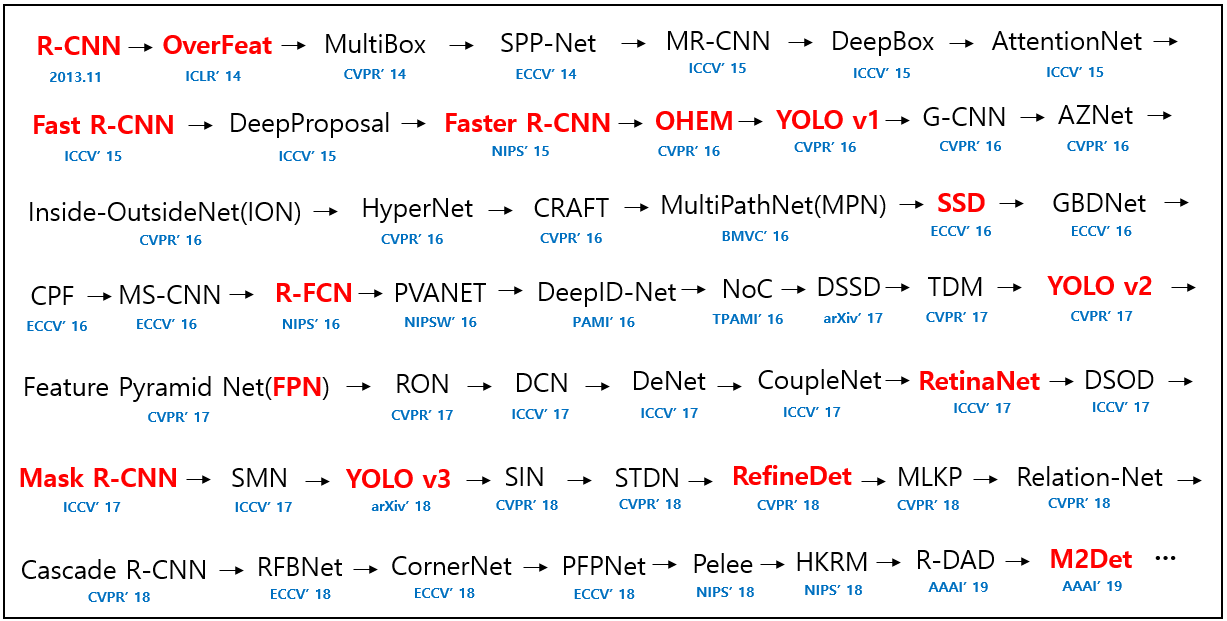
\includegraphics[width=3.44in]{list.bmp}
% where an .eps filename suffix will be assumed under latex, 
% and a .pdf suffix will be assumed for pdflatex; or what has been declared
% via \DeclareGraphicsExtensions.
\caption{2013至2019深度学习目标检测发展}
\end{figure}

在这个基础上,一系列技术也得到了进步[5]:
\begin{figure}[h]
\centering
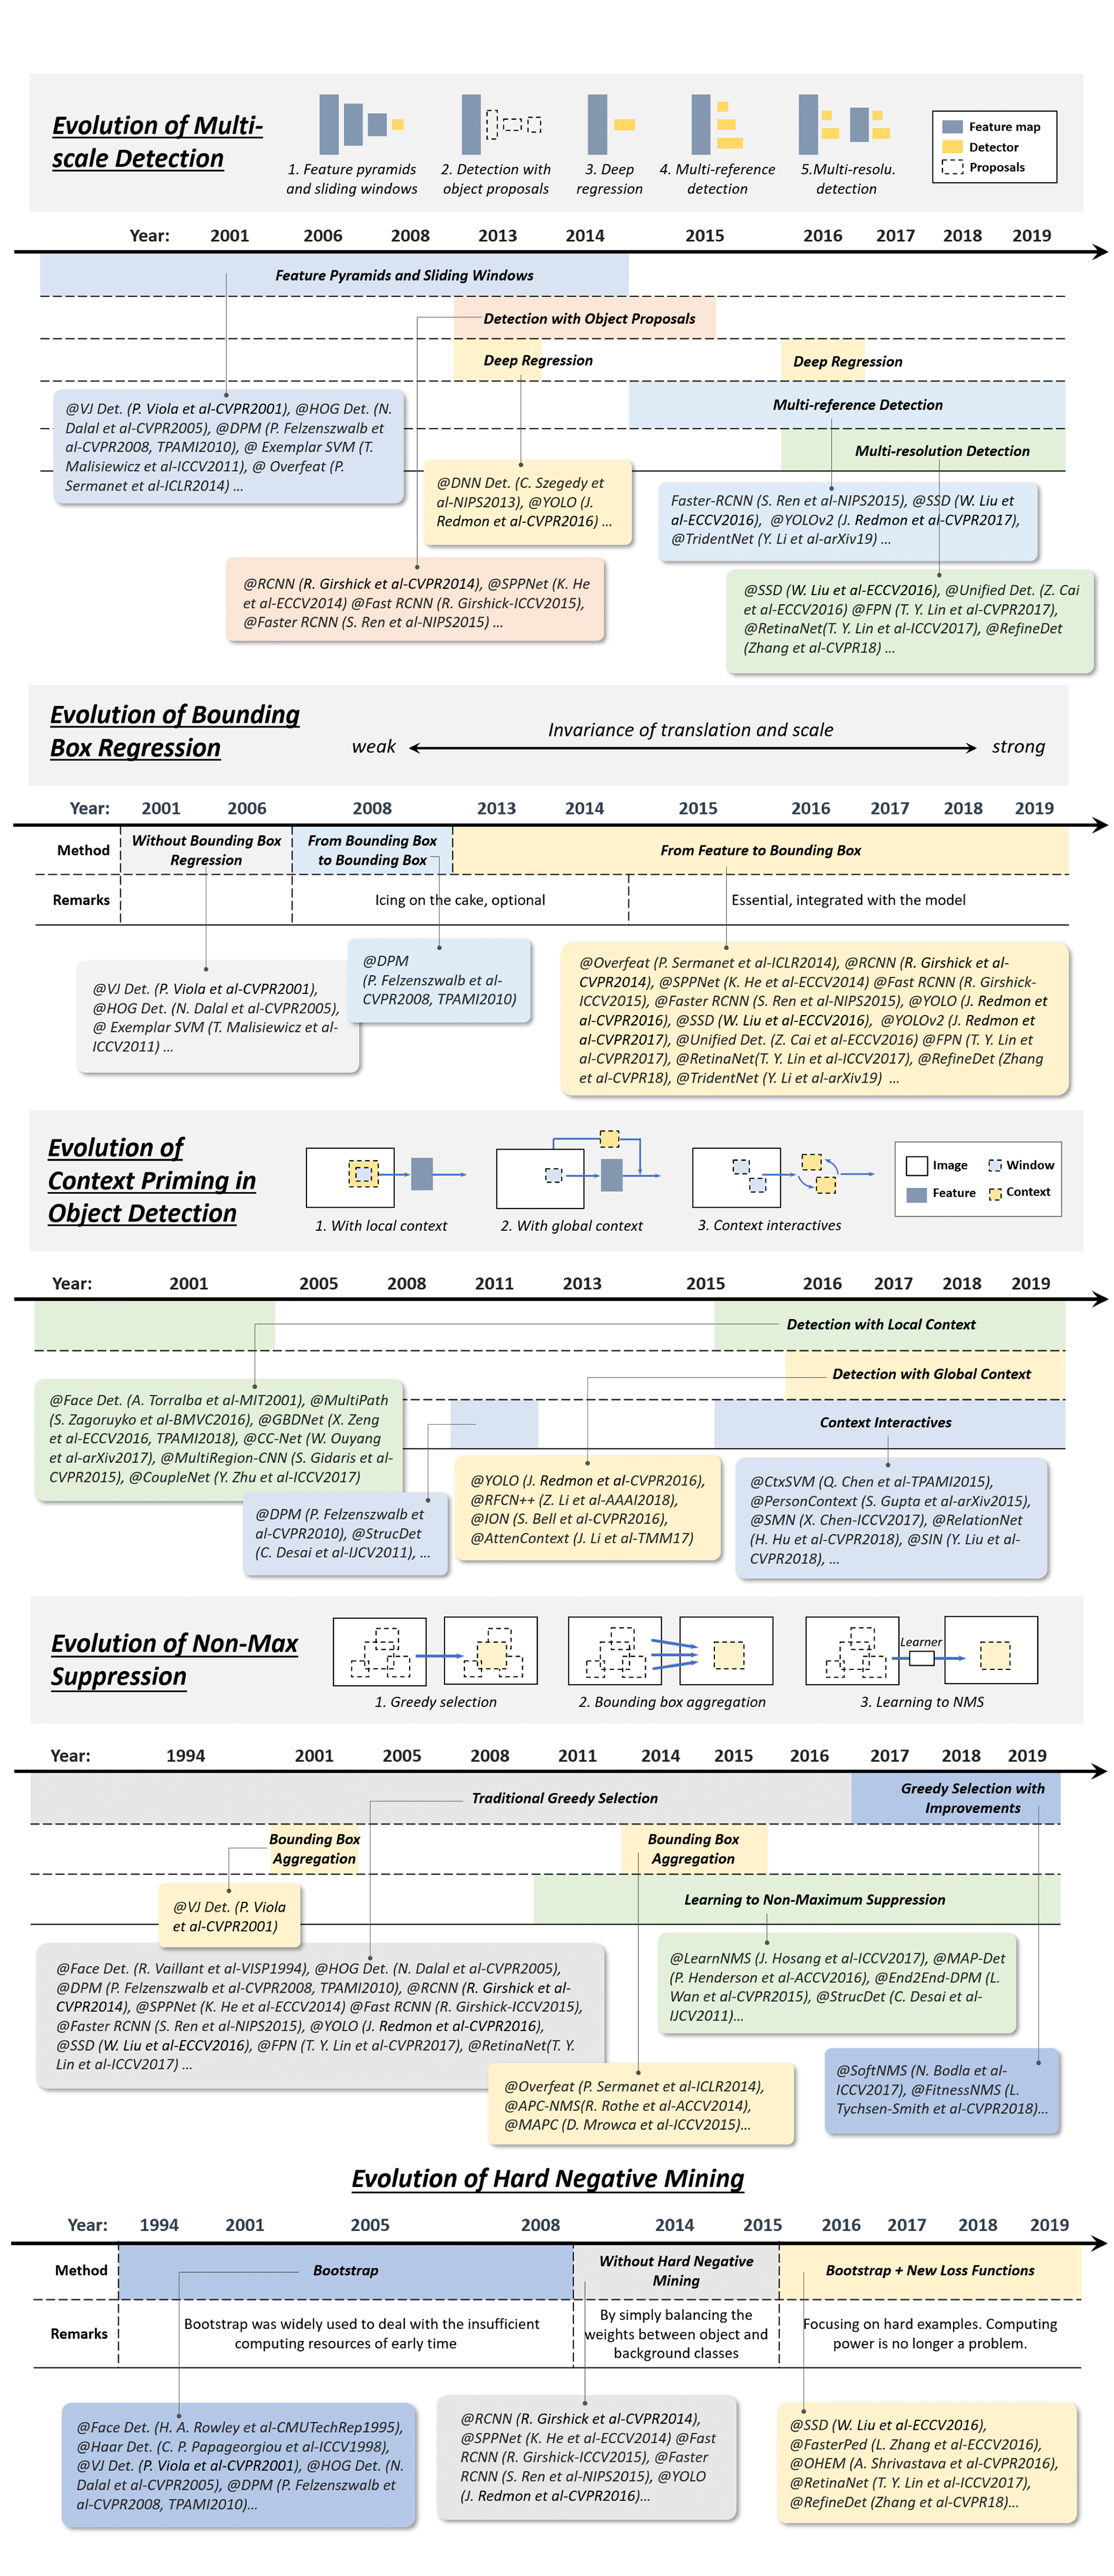
\includegraphics[width=2.6in]{update.bmp}
% where an .eps filename suffix will be assumed under latex, 
% and a .pdf suffix will be assumed for pdflatex; or what has been declared
% via \DeclareGraphicsExtensions.
\caption{Evolution of techniques in object detection from 2001 to 2019}
\end{figure}

\subsection{本文贡献}
本文利目标检测深度学习技术检测对人脸口罩进行识别。本文构建了 3 种不同的模型,分别是一阶段的SSD以及二阶段的Faster RCNN以及Focal Loss,来做口罩目标的检测。同时也针对结果最优秀的Faster RCNN做了一个电脑摄像头的实时检测。

\section{数据整理}
采用数据为公开数据集:AIZOO 的 FaceMaskDetection。

AIZOO 的 FaceMaskDetection数据集(https://github.com/AIZOOTech/FaceMaskDetection)开源了人脸口罩检测的主流框架的相应模型,并提供了相应的推理代码。该作者开源了如表格所示 的 7,959 张人脸标注图片,数据集来自于 WIDER Face 和 MAFA 数据集, 并重新修改了标注和校验。

我们使用的AIZOO数据集,可以发现该数据集有两类的数据,分别为口罩和非口罩人像,且数据相对平衡,数据集包含对每张照片的注释,注释信息包含图片的类别、目标的位置,该数据集适合作为训练与测试,该数据分布如下:
\begin{figure}[h]
\centering
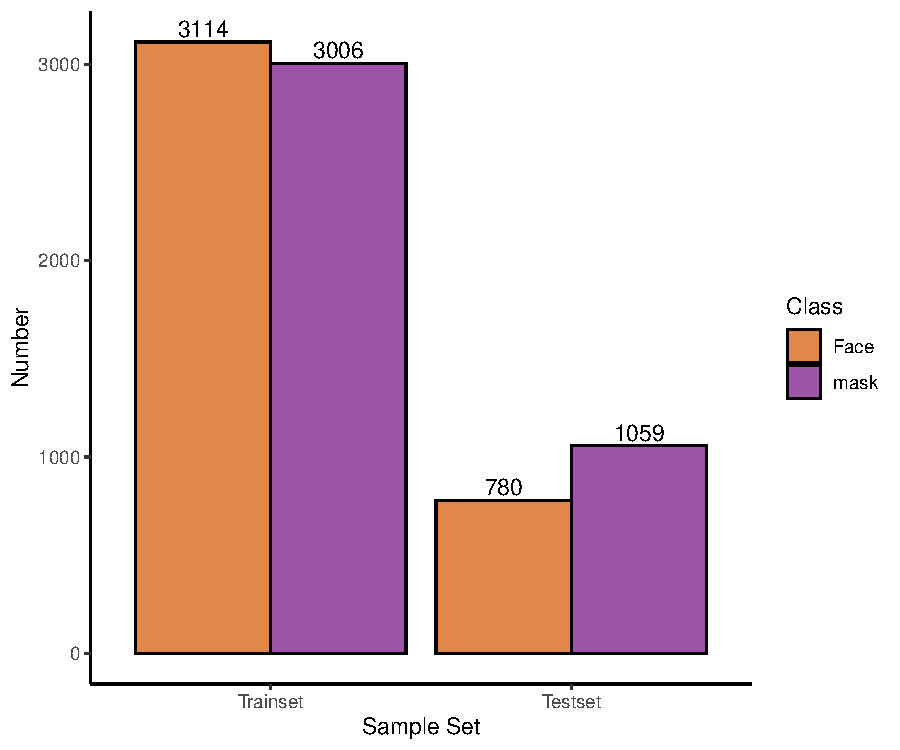
\includegraphics[width=3.44in]{Dataset.pdf}
% where an .eps filename suffix will be assumed under latex, 
% and a .pdf suffix will be assumed for pdflatex; or what has been declared
% via \DeclareGraphicsExtensions.
\caption{数据集分布可视化}
\end{figure}

在把数据应用在模型训练之前,我们务必要搞清楚要使用的标签类别与格式。主要的标签类别有Bounding Boxes、Polygonal Segmentation、Semantic Segmentation以及3D cuboids,在此一模型我们想当然用的就是用得最广泛的Bounding boxes的格式,而刚好AIZOO的数据类型也是属于这一类。在数据标签格式方面的话,AIZOO是属于Pascal VOC的标签格式,而我们在SSD使用便是这一类型;在Faster RCNN以及Focal Loss则是采用了COCO的标签格式。之所以会采用两种不同的数据格式,这是因为考虑到原模型使用了这样的标签格式,为了避免成果相差太大,我们采用了符合原模型的数据类型。

在数据整理的主要工作,便是要把Pascal VOC转换到COCO 。Pascal VOC格式是一个照片对应一个同名的xml文件,而COCO则是所有照片对应一个json文件。在转换过程中也有发现一些错字,比如face\_mask打成了face\_nask。在格式转换过程中,最大的难点在于原文件的数据格式并不一致,有者少了pascal voc的path的数据,有者则是没有图像大小的数据,而且数字序号并不统一,这些都是必须要解决的。毕竟COCO格式是在假定名称后面的数字序号是不重复的,因此可以直接通过序号来搜索资料。在转换过程中,统一把path的资料只留下图像的名称,序号也重新计算,格式转换是通过python完成,也一并附在参考代码里了。

\section{模型设计}
\subsection{SSD}
使用了SSD类型的架构,本模型输入大小为260x260,主干网络只有8个卷积层,加上定位和分类层,一共只有24层(每层的通道数目基本都是32、64、128),只有101.5万参数。八个卷积层是主干网络,也就是特征提取层,20层是定位和分类层。训练目标检测模型,最重要的合理的设置anchor的大小和宽高比,笔通过统计数据集的目标物体的宽高比和大小来设置anchor的大小和宽高比,因为人脸的一般是长方形的,而很多图片是比较宽的,人脸的宽度和高度归一化后,有很多图片的高度是宽度的2倍甚至更大。从上图也可以看出,归一化后的人脸高宽比集中在1\~2.5之间。根据数据的分布,我们将五个定位层的anchor的宽高比统一设置为1,0.62, 0.42。(转换为高宽比,也就是约1,1.6:1,2.4:1)。

为了避免使用手挡住嘴巴就会欺骗部分口罩检测系统的情况,在数据集中加入了部分嘴巴被手捂住的数据,另外在训练的过程中,随机的往嘴巴部分粘贴一些其他物体的图片,从而避免模型认为只要露出嘴巴的就是没戴口罩,没露出嘴巴的就是带口罩这个问题,通过这两个规避方法,解决了非口罩遮挡物被当作口罩的误判。后处理部分主要就是非最大抑制(NMS),我们使用了单类的NMS,也就是戴口罩人脸和不戴口罩人脸两个类别一起做NMS,从而提高速度。

迭代下模型Loss如下:
\begin{figure}[h]
\centering
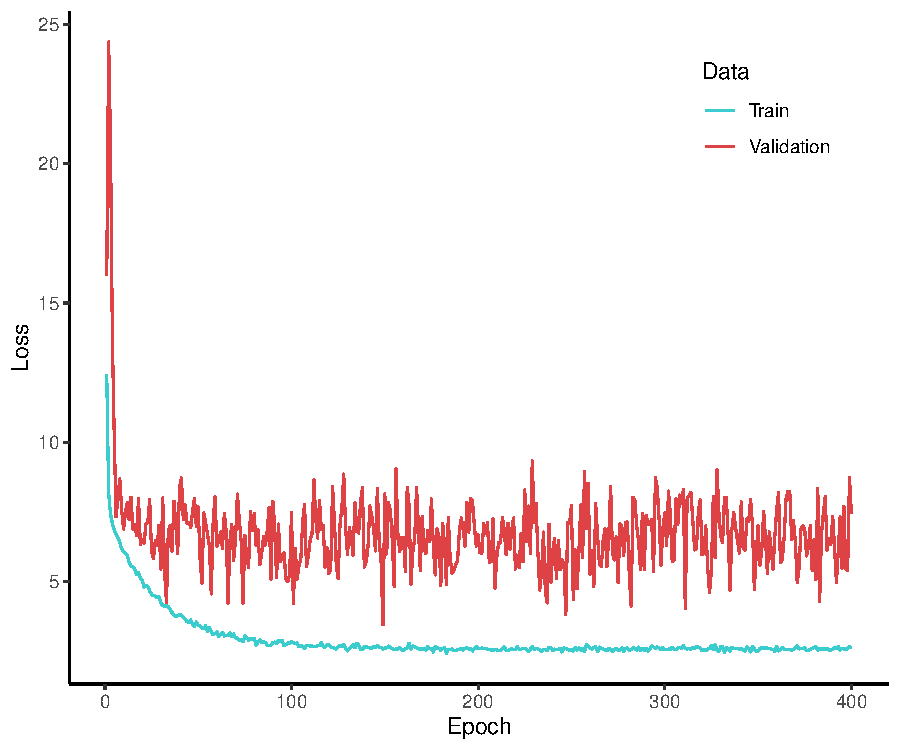
\includegraphics[width=3.44in]{Ssdloss.pdf}
% where an .eps filename suffix will be assumed under latex, 
% and a .pdf suffix will be assumed for pdflatex; or what has been declared
% via \DeclareGraphicsExtensions.
\caption{数据集分布可视化}
\end{figure}
\section{实验设计及结果}
数据集将训练集分为训练样本和验证样本,并对测试集中的样本进行测试。

下表中展示各个模型每个类别的 mAP@.5, mAP@.7, mAP@.9, mAP@[.5:.95]。
\begin{table}[!htbp]
\caption{不同模型下的mAP}  
\begin{center}  
\begin{tabular}{|l|l|l|l|l|l|}  
\hline
$Model$ & $Class$ & $mAP@.5$ & $mAP@.7$ & $mAP@.9$ & $mAP@[.5:.95]$ \\ \hline
\multirow{2}{*}{\makecell[c]{SSD}}
 & \makecell[c]{Mask} & \makecell[c]{0.86} & \makecell[c]{0.78} & \makecell[c]{0.22} & \makecell[c]{0.61}\\ \cline{2-6}
 & \makecell[c]{Face} & \makecell[c]{0.81} & \makecell[c]{0.78} & \makecell[c]{0.29} & \makecell[c]{0.63}\\ \hline

\multirow{2}{*}{\makecell[c]{Focal Loss}}
& \makecell[c]{Mask} & \makecell[c]{0.90} & \makecell[c]{0.78} & \makecell[c]{0.14} & \makecell[c]{0.59}\\ \cline{2-6}
& \makecell[c]{Face} & \makecell[c]{0.87} & \makecell[c]{0.84} & \makecell[c]{0.34} & \makecell[c]{0.69}\\ \hline

\multirow{2}{*}{\makecell[c]{Faster RCNN}}
& \makecell[c]{Mask} & \makecell[c]{0.91} & \makecell[c]{0.82} & \makecell[c]{0.25} & \makecell[c]{0.65}\\ \cline{2-6}
& \makecell[c]{Face} & \makecell[c]{0.91} & \makecell[c]{0.89} & \makecell[c]{0.47} & \makecell[c]{0.75}\\ \hline 
\end{tabular}  
\end{center}  
\end{table}

SSD模型下IoU 阈值取 0.5, 0.7, 0.9 时每类的 Precision-Recall 曲线如下:
\begin{figure}[h]
\centering
\includegraphics[width=3.44in]{ssdResult.bmp}
% where an .eps filename suffix will be assumed under latex, 
% and a .pdf suffix will be assumed for pdflatex; or what has been declared
% via \DeclareGraphicsExtensions.
\caption{SSD模型的Precision-Recall 曲线(左侧从上到下分别是口罩目标检测在IoU=0.5、0.7、0.9时的Precision-Recall 曲线;右侧为脸目标检测。)}
\end{figure}

\begin{figure}[h]
\centering
\includegraphics[width=3.44in]{FlResult.bmp}
% where an .eps filename suffix will be assumed under latex, 
% and a .pdf suffix will be assumed for pdflatex; or what has been declared
% via \DeclareGraphicsExtensions.
\caption{Focal Loss模型的Precision-Recall 曲线(左侧从上到下分别是口罩目标检测在IoU=0.5、0.7、0.9时的Precision-Recall 曲线;右侧为脸目标检测。)}
\end{figure}

\begin{figure}[h]
\centering
\includegraphics[width=3.44in]{Frcnn.bmp}
% where an .eps filename suffix will be assumed under latex, 
% and a .pdf suffix will be assumed for pdflatex; or what has been declared
% via \DeclareGraphicsExtensions.
\caption{Faster RCNN模型的Precision-Recall 曲线(左侧从上到下分别是口罩目标检测在IoU=0.5、0.7、0.9时的Precision-Recall 曲线;右侧为脸目标检测。)}
\end{figure}

\section{实验结果分析}
SSD模型结构:
\begin{figure}[h]
\centering
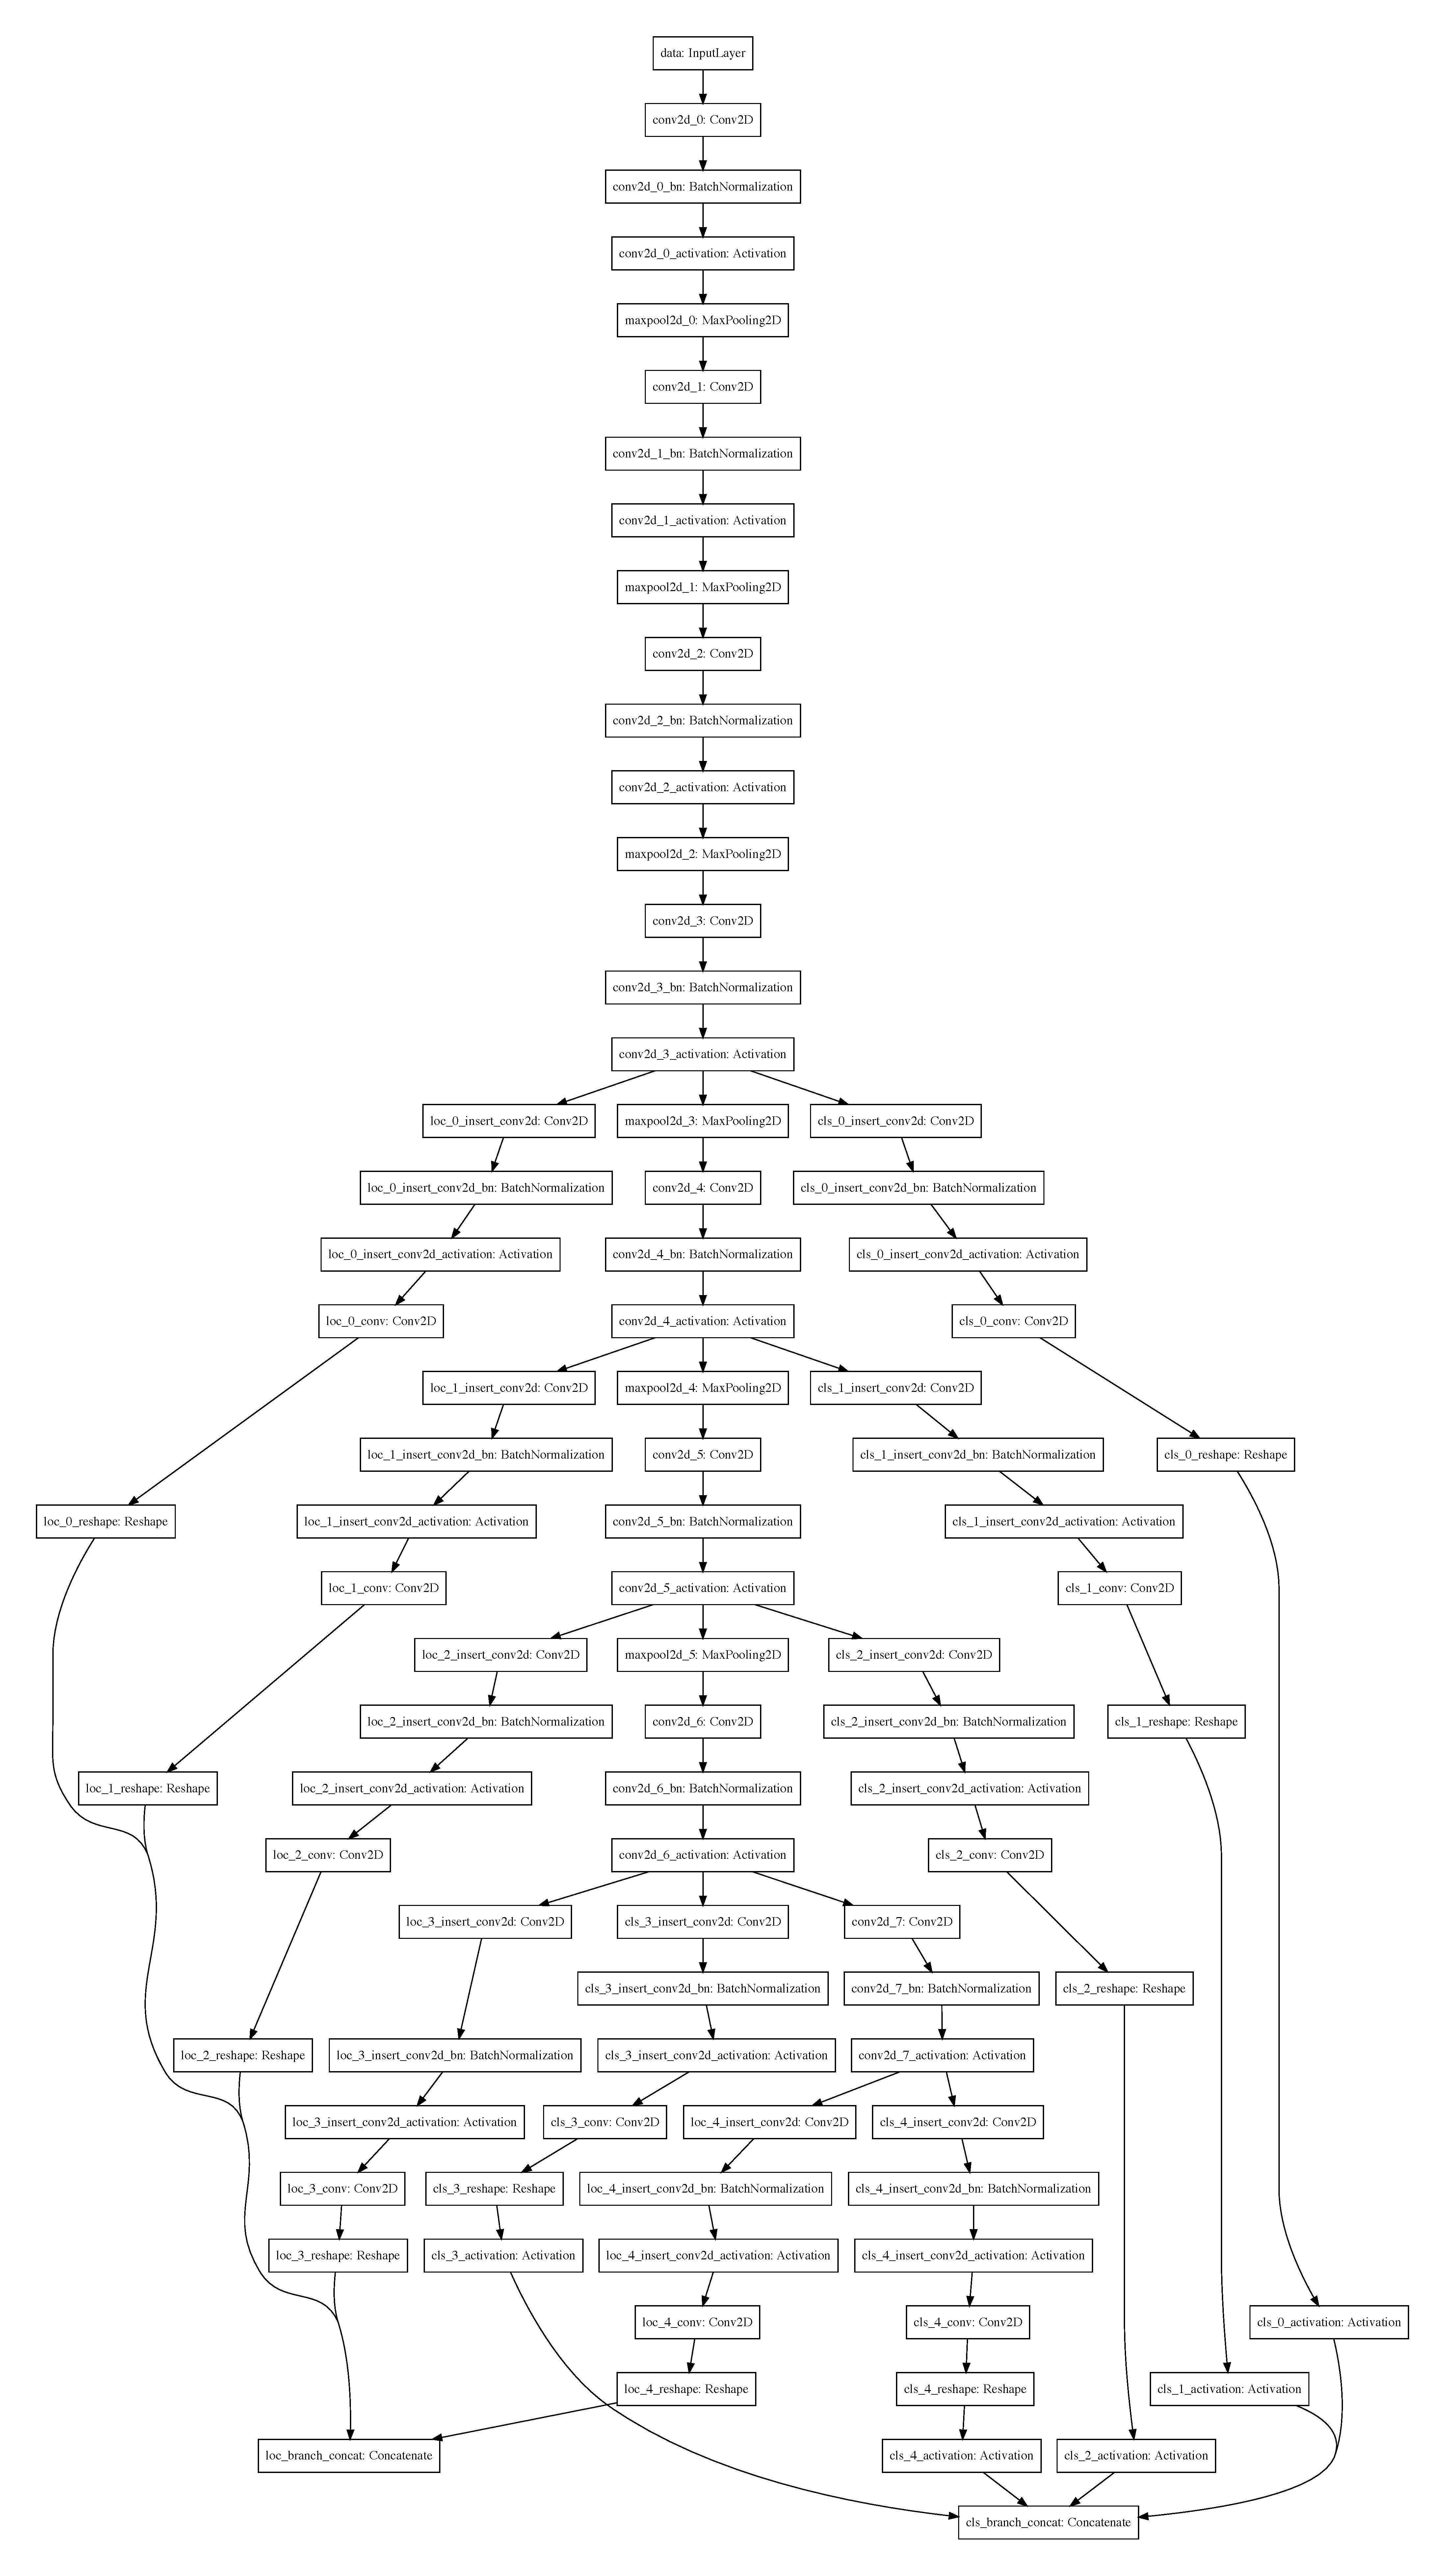
\includegraphics[width=3.44in]{modelgraph.pdf}
% where an .eps filename suffix will be assumed under latex, 
% and a .pdf suffix will be assumed for pdflatex; or what has been declared
% via \DeclareGraphicsExtensions.
\caption{SSD网络结构}
\end{figure}

不同模型的检测时间不同,对测试集的所有图片进行测试,再进行平均可以发现SSD模型的检测时间最短,其次是Focal Loss,最长的是Faster RCNN:
\begin{figure}[h]
\centering
\includegraphics[width=3.44in]{time.pdf}
% where an .eps filename suffix will be assumed under latex, 
% and a .pdf suffix will be assumed for pdflatex; or what has been declared
% via \DeclareGraphicsExtensions.
\caption{不同模型检测的时间}
\end{figure}

\section{小组成员贡献}
郑家瀚:

姚非凡:
\section{参考代码}
见附件中。
\section{结论}
通过对口罩进行目标检测,发现三种模型的检测结果中,Faster RCNN的准确率最高,不仅如此,其对脸的目标检测也最优。时间上SSD最快,但对脸的目标检测最为不佳。
% needed in second column of first page if using \IEEEpubid
%\IEEEpubidadjcol


% An example of a floating figure using the graphicx package.
% Note that \label must occur AFTER (or within) \caption.
% For figures, \caption should occur after the \includegraphics.
% Note that IEEEtran v1.7 and later has special internal code that
% is designed to preserve the operation of \label within \caption
% even when the captionsoff option is in effect. However, because
% of issues like this, it may be the safest practice to put all your
% \label just after \caption rather than within \caption{}.
%
% Reminder: the "draftcls" or "draftclsnofoot", not "draft", class
% option should be used if it is desired that the figures are to be
% displayed while in draft mode.
%
%\begin{figure}[!t]
%\centering
%\includegraphics[width=2.5in]{myfigure}
% where an .eps filename suffix will be assumed under latex, 
% and a .pdf suffix will be assumed for pdflatex; or what has been declared
% via \DeclareGraphicsExtensions.
%\caption{Simulation Results.}
%\label{fig_sim}
%\end{figure}

% Note that IEEE typically puts floats only at the top, even when this
% results in a large percentage of a column being occupied by floats.


% An example of a double column floating figure using two subfigures.
% (The subfig.sty package must be loaded for this to work.)
% The subfigure \label commands are set within each subfloat command,
% and the \label for the overall figure must come after \caption.
% \hfil is used as a separator to get equal spacing.
% Watch out that the combined width of all the subfigures on a 
% line do not exceed the text width or a line break will occur.
%
%\begin{figure*}[!t]
%\centering
%\subfloat[Case I]{\includegraphics[width=2.5in]{box}%
%\label{fig_first_case}}
%\hfil
%\subfloat[Case II]{\includegraphics[width=2.5in]{box}%
%\label{fig_second_case}}
%\caption{Simulation results.}
%\label{fig_sim}
%\end{figure*}
%
% Note that often IEEE papers with subfigures do not employ subfigure
% captions (using the optional argument to \subfloat[]), but instead will
% reference/describe all of them (a), (b), etc., within the main caption.


% An example of a floating table. Note that, for IEEE style tables, the 
% \caption command should come BEFORE the table. Table text will default to
% \footnotesize as IEEE normally uses this smaller font for tables.
% The \label must come after \caption as always.
%
%\begin{table}[!t]
%% increase table row spacing, adjust to taste
%\renewcommand{\arraystretch}{1.3}
% if using array.sty, it might be a good idea to tweak the value of
% \extrarowheight as needed to properly center the text within the cells
%\caption{An Example of a Table}
%\label{table_example}
%\centering
%% Some packages, such as MDW tools, offer better commands for making tables
%% than the plain LaTeX2e tabular which is used here.
%\begin{tabular}{|c||c|}
%\hline
%One & Two\\
%\hline
%Three & Four\\
%\hline
%\end{tabular}
%\end{table}


% Note that IEEE does not put floats in the very first column - or typically
% anywhere on the first page for that matter. Also, in-text middle ("here")
% positioning is not used. Most IEEE journals use top floats exclusively.
% Note that, LaTeX2e, unlike IEEE journals, places footnotes above bottom
% floats. This can be corrected via the \fnbelowfloat command of the
% stfloats package.
% use section* for acknowledgement
% \section*{Acknowledgment}


% The authors would like to thank...


% Can use something like this to put references on a page
% by themselves when using endfloat and the captionsoff option.
\ifCLASSOPTIONcaptionsoff
  \newpage
\fi



% trigger a \newpage just before the given reference
% number - used to balance the columns on the last page
% adjust value as needed - may need to be readjusted if
% the document is modified later
%\IEEEtriggeratref{8}
% The "triggered" command can be changed if desired:
%\IEEEtriggercmd{\enlargethispage{-5in}}

% references section

% can use a bibliography generated by BibTeX as a .bbl file
% BibTeX documentation can be easily obtained at:
% http://www.ctan.org/tex-archive/biblio/bibtex/contrib/doc/
% The IEEEtran BibTeX style support page is at:
% http://www.michaelshell.org/tex/ieeetran/bibtex/
%\bibliographystyle{IEEEtran}
% argument is your BibTeX string definitions and bibliography database(s)
%\bibliography{IEEEabrv,../bib/paper}
%
% <OR> manually copy in the resultant .bbl file
% set second argument of \begin to the number of references
% (used to reserve space for the reference number labels box)
\begin{thebibliography}{1}
\bibitem{IEEEhowto:kopka}
Redmon, J. , Divvala, S. , Girshick, R. , \& Farhadi, A. . (2015). You only look once: unified, real-time object detection.
\bibitem{IEEEhowto:kopka}
Liu, W. , Anguelov, D. , Erhan, D. , Szegedy, C. , Reed, S. , \& Fu, C. Y. , et al. (2016). Ssd: single shot multibox detector.
\bibitem{IEEEhowto:kopka}
Girshick, R. , Donahue, J. , Darrell, T. , \& Malik, J. . (2013). Rich feature hierarchies for accurate object detection and semantic segmentation.
\bibitem{IEEEhowto:kopka}
Ren, S. , He, K. , Girshick, R. , \& Sun, J. . (2015). Faster r-cnn: towards real-time object detection with region proposal networks. IEEE Transactions on Pattern Analysis and Machine Intelligence.
\bibitem{IEEEhowto:kopka}
Zou, Z. , Shi, Z. , Guo, Y. , \& Ye, J. . (2019). Object detection in 20 years: a survey.
\end{thebibliography}

% biography section
% 
% If you have an EPS/PDF photo (graphicx package needed) extra braces are
% needed around the contents of the optional argument to biography to prevent
% the LaTeX parser from getting confused when it sees the complicated
% \includegraphics command within an optional argument. (You could create
% your own custom macro containing the \includegraphics command to make things
% simpler here.)
%\begin{IEEEbiography}[{\includegraphics[width=1in,height=1.25in,clip,keepaspectratio]{mshell}}]{Michael Shell}
% or if you just want to reserve a space for a photo:

% \begin{IEEEbiography}{Michael Shell}
% Biography text here.
% \end{IEEEbiography}

% % if you will not have a photo at all:
% \begin{IEEEbiographynophoto}{John Doe}
% Biography text here.
% \end{IEEEbiographynophoto}

% % insert where needed to balance the two columns on the last page with
% % biographies
% %\newpage

% \begin{IEEEbiographynophoto}{Jane Doe}
% Biography text here.
% \end{IEEEbiographynophoto}

% You can push biographies down or up by placing
% a \vfill before or after them. The appropriate
% use of \vfill depends on what kind of text is
% on the last page and whether or not the columns
% are being equalized.

%\vfill

% Can be used to pull up biographies so that the bottom of the last one
% is flush with the other column.
%\enlargethispage{-5in}



% that's all folks
\end{document}